\subsection{Perturbation of motion in a constant field}

From \cref{fig:weakcomparison} we saw that instead of perturbing a linear Hamiltonian, we can try perturbing a Hamiltonian for a uniform magnetic field in the plane. If $R$ is the radius of the magnetic disks, $b$ the strength of the field, $L$ the Larmor radius for $b$, and likewise for $\hat L$ and $\hat b$, we proposed a relation $\hat b = \pi R^2b$. 



To test the validity of the relation, we give two tests, the results of which can be found in \cref{fig:modeling}. In \cref{subfig:3dfitting} we generated data varying both $R$ and $b$, and fit a general cubic of the form:
\begin{align*}
a_0 + a_1R + a_2b + a_3R^2 + a_4Rb + a_5b^2 + a_6R^3 +a_7R^2b+a_8Rb^2+a_9b^3=\hat b =1/\hat L,
\end{align*}
using a least-squares method. In \cref{subfig:2dfitting} the same is done but first we fix $R=1/3$ and then fit a line $a_0+a_1R^2b$.

We generated the data as follows: for $1\le i\le 50$ we sample values $(R_i, b_i)$ uniformly in the range $[0.25,0.45]\times[10^{-10},10^{-6}]$ (in the second test $R_i=1/3$). For $R_i, b_i$ we uniformly sample initial conditions $X_{ij}$ with $1\le j\le 20$. We fit a circle to the trajectory of each $X_{ij}$ and from these circles we extract the radius $\hat L_{ij}$. Finally, we take the average $\hat L_i=\sum_{j=1}^{20}\hat L_{ij}/20$. 

To fit the circles we use the method of I.\,Coope which uses a change of coordinates to bring a non-linear least squares problem to the form of a linear problem. The set up and advantages of this method are discussed in \cite{Coope93}, and our use of it can be viewed at [??]. 

\begin{figure}[!ht]
\centering
\begin{subfigure}[!th]{0.49\textwidth}
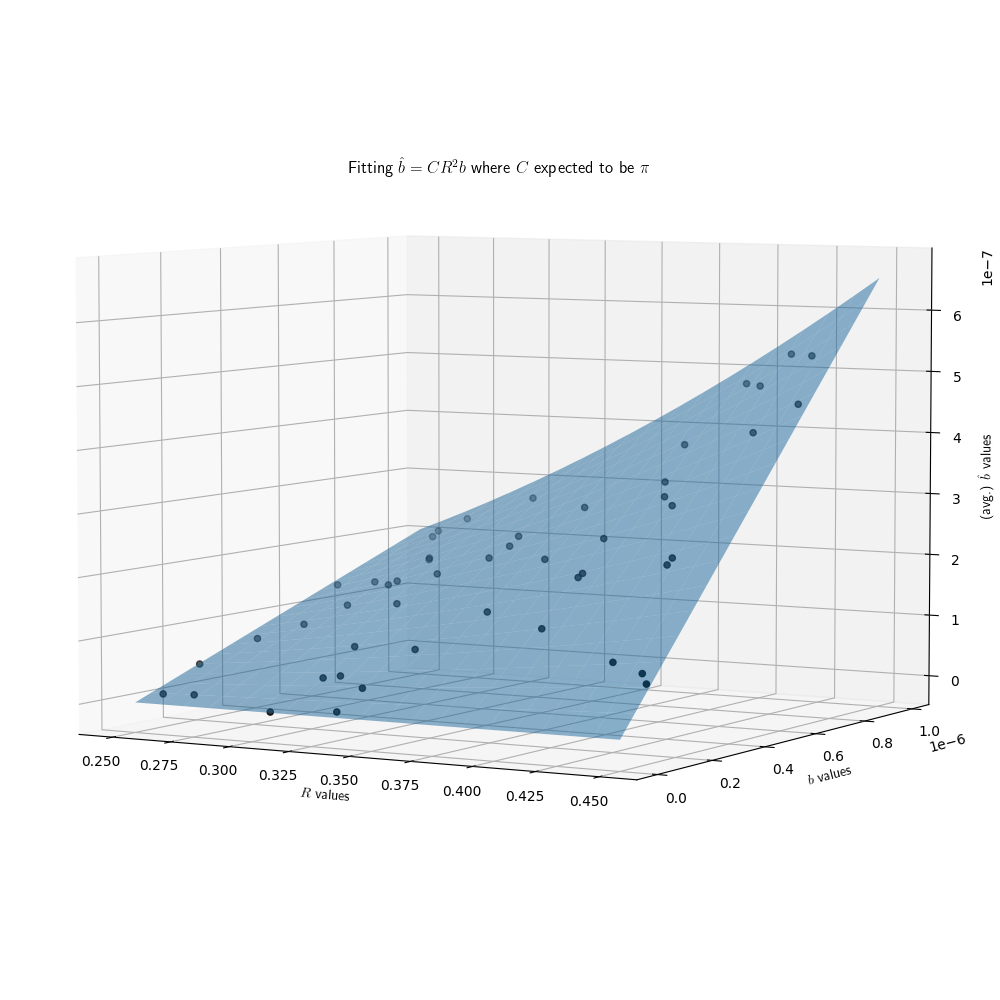
\includegraphics[width=\textwidth, trim={0 5cm 0 4cm}, clip]{fig8.png}
\caption{Fitting a cubic surface}
\label{subfig:3dfitting}
\end{subfigure}
%
\begin{subfigure}[!th]{0.49\textwidth}
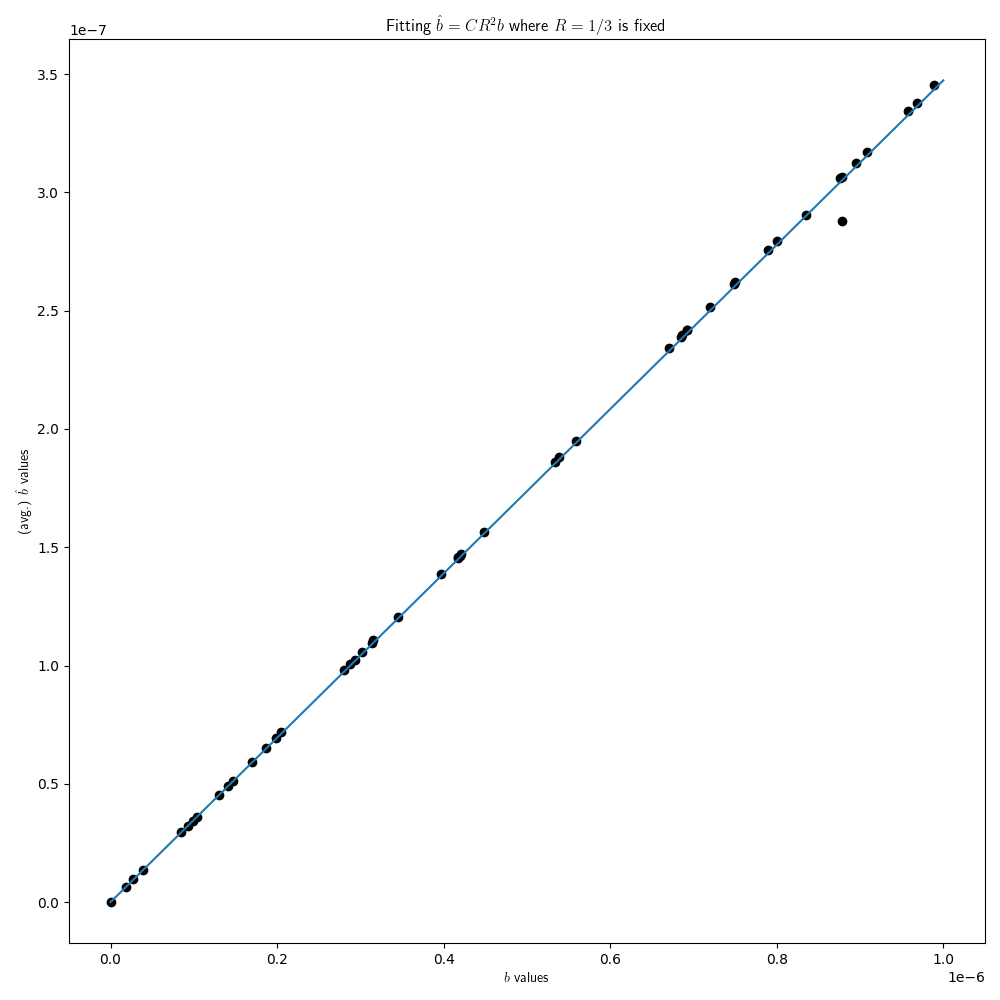
\includegraphics[width=\textwidth]{fig9.png}
\caption{Fitting a line}
\label{subfig:2dfitting}
\end{subfigure}
\caption{Fitting surfaces and lines to data to determine the parameter in our model.}
\label{fig:modeling}
\end{figure}

The coefficients of the fitted cubic surface in \cref{subfig:3dfitting} come out to
\begin{align*}
a_0&\approx  6.7\cdot10^{-8},	&
a_1&\approx -6.2\cdot10^{-7},	&
a_2&\approx  6.7\cdot10^{-3},\\
a_3&\approx  1.9\cdot10^{-6},	&
a_4&\approx -5.3\cdot10^{-2},	&
a_5&\approx -1.9\cdot10^{+2},\\
a_6&\approx -1.8\cdot10^{-6},	&
a_7&\approx  3.2,				&
a_8&\approx  -6.6\cdot10^{+1},\\
a_9&\approx  -3.0\cdot10^{-4},
\end{align*} 
the values of $a_0$ to $a_4$, $a_6$ and $a_9$ are negligible as expected, likewise $a_7\approx\pi$. We notice that $a_5$ and $a_8$ are quite large but we reason that the contribution of their respective monomial term is still small, since both contain a factor of $b^2$ which has an order of magnitude at most $10^{-6}$. The coefficients of the fitted line in \cref{subfig:2dfitting} are $a_0\approx 4.4\cdot10^{10}$ and $a_1\approx3.12$, which can be explained in the same way. So, the relation $\hat b =\pi R^2b$ seems valid, and this motivates perturbing a uniform magnetic field into the bump field

Overall, the results show that our assumptions are plausible, we approximately see $\pi$ in the coefficient. The results are not as precise as desired but that can be due to randomly choosing the initial conditions for the trajectories. The circular trajectories correspond to invariant tori, and since not all tori are preserved under the perturbation, we expect that, chosen at random, some trajectories will not follow closely a circular path. Similarly, the chosen range for sampling $R$ and $b$ could be too large, though in tests we made that we omit here, we noticed that the relation holds more or less for a wider range of $[0.1, 0.45]\times[10^{-16}, 10^{-2}]$.

